 \documentclass[journal,12pt,twocolumn]{IEEEtran}
\usepackage{graphicx}
\graphicspath{{./figs/}}{}
\usepackage{amsmath,amssymb,amsfonts,amsthm}
\newcommand{\myvec}[1]{\ensuremath{\begin{pmatrix}#1\end{pmatrix}}}

\let\vec\mathbf

\title{
Matrix-Lines
}
\author{Jyothsna Paluchuri-FWC22059\\}
\begin{document}
\maketitle
\tableofcontents
\bigskip
\section{Problem Statement}
Find the slope of a line,which passes through the origin and the mid point of the line segment joining the points P(0,-4) and B(8,0)\\
\section{Construction}
\begin{figure}[h]
    \centering
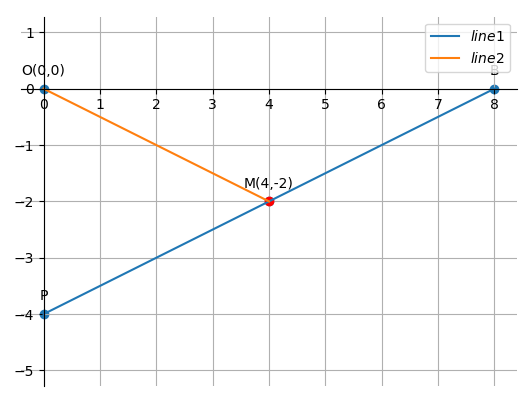
\includegraphics[width=\columnwidth]{line.png}
    \caption{Equation of the slope}
    \label{fig:my_label}
\end{figure}
\vspace{2cm}
\begin{table}[h]
    \centering
    \begin{tabular}{|c|c|c|c|}
       \hline
       \textbf{Symbol}&\textbf{Value}&\textbf{Description}  \\
       \hline
	    $\vec{P}$ & $\myvec{
		    0\\
		    -4}$
	    & Point on Y-axis\\
        \hline
	    $\vec{B}$ & $\myvec{8\\0}$
 & Point on X-axis\\
        \hline
	    $\vec{0}$ & $\myvec{0\\0}$
 & Origin\\
        \hline
    \end{tabular}
    \caption{Parameters}
    \label{tab:my_label}
\end{table}


\section{Solution}
Given that resultant line passes through origin and mid point of the line segment joining point P(0,-4) and B(8,0) \\
\\
\\
given ${\vec{P}}$=$\myvec{
  0\\
  -4}$
 , ${\vec{B}}$=$\myvec{
  8\\
  0}$
  
  
\textbf{The mid point of PB line:} \\
\begin{align}
\implies\vec{M} &=\frac{1}{2}(\vec{P}+\vec{B})
\end{align}
\begin{align}
\implies\vec{M} &= \begin{pmatrix}4 \\ -2 \\ \end{pmatrix} 
\end{align}
\\
\textbf{The direction vector of line joining two points $\vec{O}$,$\vec{M}$ is given by}
\begin{align}
\implies\vec{m}&=\vec{O}-\vec{M}
\end{align}
\begin{align}
\implies\vec{m} &= \begin{pmatrix}4 \\ -2 \\ \end{pmatrix}
\end{align}
\textbf{By simplifying eq(4),we get}
\begin{align}
\implies\vec{m} &= \begin{pmatrix}1 \\ -0.5 \\ \end{pmatrix}
\end{align}
\textbf{The direction vector of a line expressed as}
\begin{align}
\implies\vec{m} &= \begin{pmatrix}1 \\ m \\ \end{pmatrix}
\end{align}

\textbf{By solving equation (5) and (6),we get the slope of $\vec{O}$ $\vec{M}$ line}
\begin{align}
        \boxed{m=-0.5}
 \end{align}

\section{Software}
Download the following code using,
\begin{table}[h]
    \centering
    \begin{tabular}{|c|}
    \hline \\
   https://github.com/jyothsna777/jyothsna-fwc.git  \\
         \\
\hline
    \end{tabular}
\end{table}
\\
and execute the code by using command
\begin{center}
\textbf{Python3 lines.py}\\
\end{center}

\section{Conclusion}
Hence the slope of line $\vec{O}$ $\vec{M}$ lineis $\vec{m}$=-0.5

\end{document}
